\PassOptionsToPackage{unicode=true}{hyperref} % options for packages loaded elsewhere
\PassOptionsToPackage{hyphens}{url}
%
\documentclass[]{article}
\usepackage{lmodern}
\usepackage{amssymb,amsmath}
\usepackage{ifxetex,ifluatex}
\usepackage{fixltx2e} % provides \textsubscript
\ifnum 0\ifxetex 1\fi\ifluatex 1\fi=0 % if pdftex
  \usepackage[T1]{fontenc}
  \usepackage[utf8]{inputenc}
  \usepackage{textcomp} % provides euro and other symbols
\else % if luatex or xelatex
  \usepackage{unicode-math}
  \defaultfontfeatures{Ligatures=TeX,Scale=MatchLowercase}
\fi
% use upquote if available, for straight quotes in verbatim environments
\IfFileExists{upquote.sty}{\usepackage{upquote}}{}
% use microtype if available
\IfFileExists{microtype.sty}{%
\usepackage[]{microtype}
\UseMicrotypeSet[protrusion]{basicmath} % disable protrusion for tt fonts
}{}
\IfFileExists{parskip.sty}{%
\usepackage{parskip}
}{% else
\setlength{\parindent}{0pt}
\setlength{\parskip}{6pt plus 2pt minus 1pt}
}
\usepackage{hyperref}
\hypersetup{
            pdftitle={Milestone 03 - Group 09},
            pdfauthor={Daniel Hadley, Kristina Wright},
            pdfborder={0 0 0},
            breaklinks=true}
\urlstyle{same}  % don't use monospace font for urls
\usepackage[margin=1in]{geometry}
\usepackage{color}
\usepackage{fancyvrb}
\newcommand{\VerbBar}{|}
\newcommand{\VERB}{\Verb[commandchars=\\\{\}]}
\DefineVerbatimEnvironment{Highlighting}{Verbatim}{commandchars=\\\{\}}
% Add ',fontsize=\small' for more characters per line
\usepackage{framed}
\definecolor{shadecolor}{RGB}{248,248,248}
\newenvironment{Shaded}{\begin{snugshade}}{\end{snugshade}}
\newcommand{\AlertTok}[1]{\textcolor[rgb]{0.94,0.16,0.16}{#1}}
\newcommand{\AnnotationTok}[1]{\textcolor[rgb]{0.56,0.35,0.01}{\textbf{\textit{#1}}}}
\newcommand{\AttributeTok}[1]{\textcolor[rgb]{0.77,0.63,0.00}{#1}}
\newcommand{\BaseNTok}[1]{\textcolor[rgb]{0.00,0.00,0.81}{#1}}
\newcommand{\BuiltInTok}[1]{#1}
\newcommand{\CharTok}[1]{\textcolor[rgb]{0.31,0.60,0.02}{#1}}
\newcommand{\CommentTok}[1]{\textcolor[rgb]{0.56,0.35,0.01}{\textit{#1}}}
\newcommand{\CommentVarTok}[1]{\textcolor[rgb]{0.56,0.35,0.01}{\textbf{\textit{#1}}}}
\newcommand{\ConstantTok}[1]{\textcolor[rgb]{0.00,0.00,0.00}{#1}}
\newcommand{\ControlFlowTok}[1]{\textcolor[rgb]{0.13,0.29,0.53}{\textbf{#1}}}
\newcommand{\DataTypeTok}[1]{\textcolor[rgb]{0.13,0.29,0.53}{#1}}
\newcommand{\DecValTok}[1]{\textcolor[rgb]{0.00,0.00,0.81}{#1}}
\newcommand{\DocumentationTok}[1]{\textcolor[rgb]{0.56,0.35,0.01}{\textbf{\textit{#1}}}}
\newcommand{\ErrorTok}[1]{\textcolor[rgb]{0.64,0.00,0.00}{\textbf{#1}}}
\newcommand{\ExtensionTok}[1]{#1}
\newcommand{\FloatTok}[1]{\textcolor[rgb]{0.00,0.00,0.81}{#1}}
\newcommand{\FunctionTok}[1]{\textcolor[rgb]{0.00,0.00,0.00}{#1}}
\newcommand{\ImportTok}[1]{#1}
\newcommand{\InformationTok}[1]{\textcolor[rgb]{0.56,0.35,0.01}{\textbf{\textit{#1}}}}
\newcommand{\KeywordTok}[1]{\textcolor[rgb]{0.13,0.29,0.53}{\textbf{#1}}}
\newcommand{\NormalTok}[1]{#1}
\newcommand{\OperatorTok}[1]{\textcolor[rgb]{0.81,0.36,0.00}{\textbf{#1}}}
\newcommand{\OtherTok}[1]{\textcolor[rgb]{0.56,0.35,0.01}{#1}}
\newcommand{\PreprocessorTok}[1]{\textcolor[rgb]{0.56,0.35,0.01}{\textit{#1}}}
\newcommand{\RegionMarkerTok}[1]{#1}
\newcommand{\SpecialCharTok}[1]{\textcolor[rgb]{0.00,0.00,0.00}{#1}}
\newcommand{\SpecialStringTok}[1]{\textcolor[rgb]{0.31,0.60,0.02}{#1}}
\newcommand{\StringTok}[1]{\textcolor[rgb]{0.31,0.60,0.02}{#1}}
\newcommand{\VariableTok}[1]{\textcolor[rgb]{0.00,0.00,0.00}{#1}}
\newcommand{\VerbatimStringTok}[1]{\textcolor[rgb]{0.31,0.60,0.02}{#1}}
\newcommand{\WarningTok}[1]{\textcolor[rgb]{0.56,0.35,0.01}{\textbf{\textit{#1}}}}
\usepackage{longtable,booktabs}
% Fix footnotes in tables (requires footnote package)
\IfFileExists{footnote.sty}{\usepackage{footnote}\makesavenoteenv{longtable}}{}
\usepackage{graphicx,grffile}
\makeatletter
\def\maxwidth{\ifdim\Gin@nat@width>\linewidth\linewidth\else\Gin@nat@width\fi}
\def\maxheight{\ifdim\Gin@nat@height>\textheight\textheight\else\Gin@nat@height\fi}
\makeatother
% Scale images if necessary, so that they will not overflow the page
% margins by default, and it is still possible to overwrite the defaults
% using explicit options in \includegraphics[width, height, ...]{}
\setkeys{Gin}{width=\maxwidth,height=\maxheight,keepaspectratio}
\setlength{\emergencystretch}{3em}  % prevent overfull lines
\providecommand{\tightlist}{%
  \setlength{\itemsep}{0pt}\setlength{\parskip}{0pt}}
\setcounter{secnumdepth}{0}
% Redefines (sub)paragraphs to behave more like sections
\ifx\paragraph\undefined\else
\let\oldparagraph\paragraph
\renewcommand{\paragraph}[1]{\oldparagraph{#1}\mbox{}}
\fi
\ifx\subparagraph\undefined\else
\let\oldsubparagraph\subparagraph
\renewcommand{\subparagraph}[1]{\oldsubparagraph{#1}\mbox{}}
\fi

% set default figure placement to htbp
\makeatletter
\def\fps@figure{htbp}
\makeatother


\title{Milestone 03 - Group 09}
\author{Daniel Hadley, Kristina Wright}
\date{March 14, 2020}

\begin{document}
\maketitle

\hypertarget{airbnb-listings-for-barcelona}{%
\subsection{Airbnb Listings for
Barcelona}\label{airbnb-listings-for-barcelona}}

\hypertarget{introduction}{%
\subsubsection{Introduction}\label{introduction}}

Airbnb, Inc.~is a company founded in 2008 that offers an online
marketplace connecting people who offer lodging with people who require
accomodations in that locale. The company does not own any of the listed
properties and operates as a broker, collecting commissions once a
lodging is booked. As a direct competitor to hotels, we are interested
in how the users listing properties determine the price they charge.

When accomodations are offered through Airbnb, the person listing the
property is called a host, and they must provide a variety of
information about the listing including price, neighborhood, type of
accommodations offered, and the minimum number of nights a guest must
stay if they want to make a booking. In addition to information provided
by the host, Airbnb collects and disseminates information about the
listing which we use to perform our analysis.

The data is collected using public information compiled from the Airbnb
website. Specific collection techniques are not specified, though the
Inside Airbnb \href{http://insideairbnb.com/behind.html}{website} states
that it uses Open Source technologies such as D3, Boostrap, jQuery, etc.
to collect the data and much code was ``copied and pasted'' from the
internet. A major contributer to this code,
\href{http://tomslee.net/category/airbnb-data}{Tom Slee}, described it
as a ``scrape'' of the Airbnb website for each city.

\hypertarget{data-description}{%
\subsubsection{Data Description}\label{data-description}}

The \href{http://insideairbnb.com/get-the-data.html}{dataset} used in
this analysis is collected and offered by Inside Airbnb, an independent,
non-commercial project started by Murray Cox and John Morris. Their goal
is to allow people to see how Airbnb might be affecting the residential
housing market. We use the summary data for listings, since it includes
the data we are interested in exploring and is more manageable,
size-wise, than the detailed listings data.

The data used in this analysis was compiled on November 9, 2019 and
includes 20,428 Airbnb listings that travellers see when using the
Airbnb website to find accommodations in Barcelona, Spain. The table
below describes the available data for each listing in the dataset.

\begin{longtable}[]{@{}llll@{}}
\toprule
\begin{minipage}[b]{0.22\columnwidth}\raggedright
Variable Name\strut
\end{minipage} & \begin{minipage}[b]{0.22\columnwidth}\raggedright
Column Name\strut
\end{minipage} & \begin{minipage}[b]{0.22\columnwidth}\raggedright
Type of Data\strut
\end{minipage} & \begin{minipage}[b]{0.22\columnwidth}\raggedright
Description\strut
\end{minipage}\tabularnewline
\midrule
\endhead
\begin{minipage}[t]{0.22\columnwidth}\raggedright
Listing ID\strut
\end{minipage} & \begin{minipage}[t]{0.22\columnwidth}\raggedright
\texttt{id}\strut
\end{minipage} & \begin{minipage}[t]{0.22\columnwidth}\raggedright
Categorical/Numeric\strut
\end{minipage} & \begin{minipage}[t]{0.22\columnwidth}\raggedright
Numeric identifier unique to each listing\strut
\end{minipage}\tabularnewline
\begin{minipage}[t]{0.22\columnwidth}\raggedright
Name\strut
\end{minipage} & \begin{minipage}[t]{0.22\columnwidth}\raggedright
\texttt{name}\strut
\end{minipage} & \begin{minipage}[t]{0.22\columnwidth}\raggedright
Character\strut
\end{minipage} & \begin{minipage}[t]{0.22\columnwidth}\raggedright
Short title for the listing provided by the host\strut
\end{minipage}\tabularnewline
\begin{minipage}[t]{0.22\columnwidth}\raggedright
Host ID\strut
\end{minipage} & \begin{minipage}[t]{0.22\columnwidth}\raggedright
\texttt{host\_id}\strut
\end{minipage} & \begin{minipage}[t]{0.22\columnwidth}\raggedright
Categorical/Numeric\strut
\end{minipage} & \begin{minipage}[t]{0.22\columnwidth}\raggedright
Numeric identifier for the host of the listing\strut
\end{minipage}\tabularnewline
\begin{minipage}[t]{0.22\columnwidth}\raggedright
Host Name\strut
\end{minipage} & \begin{minipage}[t]{0.22\columnwidth}\raggedright
\texttt{host\_name}\strut
\end{minipage} & \begin{minipage}[t]{0.22\columnwidth}\raggedright
Categorical/String\strut
\end{minipage} & \begin{minipage}[t]{0.22\columnwidth}\raggedright
Name of the host or hosts of the listing provided by the host(s) to
Airbnb\strut
\end{minipage}\tabularnewline
\begin{minipage}[t]{0.22\columnwidth}\raggedright
Neighbourhood Group\strut
\end{minipage} & \begin{minipage}[t]{0.22\columnwidth}\raggedright
\texttt{neighbourhood\_group}\strut
\end{minipage} & \begin{minipage}[t]{0.22\columnwidth}\raggedright
Categorical/String\strut
\end{minipage} & \begin{minipage}[t]{0.22\columnwidth}\raggedright
Districts of Barcelona as determined by the coordinates of the listing
and the city's definition of its districts; this data is not the data
provided by the host\strut
\end{minipage}\tabularnewline
\begin{minipage}[t]{0.22\columnwidth}\raggedright
Neighbourhood\strut
\end{minipage} & \begin{minipage}[t]{0.22\columnwidth}\raggedright
\texttt{neighbourhood}\strut
\end{minipage} & \begin{minipage}[t]{0.22\columnwidth}\raggedright
Categorical/String\strut
\end{minipage} & \begin{minipage}[t]{0.22\columnwidth}\raggedright
Neighbourhoods of Barcelona are smaller geographical areas than
districts and are determined by the coordinates of the listing and
compared to the city's boundaries of its neighbourhoods; this data is
not the neighbourhood provided by the host\strut
\end{minipage}\tabularnewline
\begin{minipage}[t]{0.22\columnwidth}\raggedright
Latitude\strut
\end{minipage} & \begin{minipage}[t]{0.22\columnwidth}\raggedright
\texttt{latitude}\strut
\end{minipage} & \begin{minipage}[t]{0.22\columnwidth}\raggedright
Numeric\strut
\end{minipage} & \begin{minipage}[t]{0.22\columnwidth}\raggedright
Latitude coordinates of the listing\strut
\end{minipage}\tabularnewline
\begin{minipage}[t]{0.22\columnwidth}\raggedright
Longitude\strut
\end{minipage} & \begin{minipage}[t]{0.22\columnwidth}\raggedright
\texttt{longitude}\strut
\end{minipage} & \begin{minipage}[t]{0.22\columnwidth}\raggedright
Numeric\strut
\end{minipage} & \begin{minipage}[t]{0.22\columnwidth}\raggedright
Longitude coordinates of the listing\strut
\end{minipage}\tabularnewline
\begin{minipage}[t]{0.22\columnwidth}\raggedright
Type of Accommodation\strut
\end{minipage} & \begin{minipage}[t]{0.22\columnwidth}\raggedright
\texttt{room\_type}\strut
\end{minipage} & \begin{minipage}[t]{0.22\columnwidth}\raggedright
Categorical/String\strut
\end{minipage} & \begin{minipage}[t]{0.22\columnwidth}\raggedright
Type of accommodations specify whether the listing is for an entire home
or apartment, a private room in a shared home or apartment, a hotel
room, or a shared room\strut
\end{minipage}\tabularnewline
\begin{minipage}[t]{0.22\columnwidth}\raggedright
Price\strut
\end{minipage} & \begin{minipage}[t]{0.22\columnwidth}\raggedright
\texttt{price}\strut
\end{minipage} & \begin{minipage}[t]{0.22\columnwidth}\raggedright
Numeric\strut
\end{minipage} & \begin{minipage}[t]{0.22\columnwidth}\raggedright
The price per night, in euros, to book a listing\strut
\end{minipage}\tabularnewline
\begin{minipage}[t]{0.22\columnwidth}\raggedright
Minimum Stay\strut
\end{minipage} & \begin{minipage}[t]{0.22\columnwidth}\raggedright
\texttt{minimum\_nights}\strut
\end{minipage} & \begin{minipage}[t]{0.22\columnwidth}\raggedright
Numeric\strut
\end{minipage} & \begin{minipage}[t]{0.22\columnwidth}\raggedright
The minimum number of nights that a guest must reserve in order to book
a listing\strut
\end{minipage}\tabularnewline
\begin{minipage}[t]{0.22\columnwidth}\raggedright
Number of Reviews\strut
\end{minipage} & \begin{minipage}[t]{0.22\columnwidth}\raggedright
\texttt{number\_of\_reviews}\strut
\end{minipage} & \begin{minipage}[t]{0.22\columnwidth}\raggedright
Numeric\strut
\end{minipage} & \begin{minipage}[t]{0.22\columnwidth}\raggedright
The number of reviews left by guests after their stay\strut
\end{minipage}\tabularnewline
\begin{minipage}[t]{0.22\columnwidth}\raggedright
Last Review\strut
\end{minipage} & \begin{minipage}[t]{0.22\columnwidth}\raggedright
\texttt{last\_review}\strut
\end{minipage} & \begin{minipage}[t]{0.22\columnwidth}\raggedright
Date\strut
\end{minipage} & \begin{minipage}[t]{0.22\columnwidth}\raggedright
The date of the last review left by a guest\strut
\end{minipage}\tabularnewline
\begin{minipage}[t]{0.22\columnwidth}\raggedright
Reviews per Month\strut
\end{minipage} & \begin{minipage}[t]{0.22\columnwidth}\raggedright
\texttt{reviews\_per\_month}\strut
\end{minipage} & \begin{minipage}[t]{0.22\columnwidth}\raggedright
Numeric\strut
\end{minipage} & \begin{minipage}[t]{0.22\columnwidth}\raggedright
The number of reviews left by guests of a listing divided by the number
of months the listing has been active\strut
\end{minipage}\tabularnewline
\begin{minipage}[t]{0.22\columnwidth}\raggedright
Number of Listings by Host\strut
\end{minipage} & \begin{minipage}[t]{0.22\columnwidth}\raggedright
\texttt{calculated\_host\_listings\_count}\strut
\end{minipage} & \begin{minipage}[t]{0.22\columnwidth}\raggedright
Numeric\strut
\end{minipage} & \begin{minipage}[t]{0.22\columnwidth}\raggedright
A count of the number of listings under the same Host Name\strut
\end{minipage}\tabularnewline
\begin{minipage}[t]{0.22\columnwidth}\raggedright
Availability\strut
\end{minipage} & \begin{minipage}[t]{0.22\columnwidth}\raggedright
\texttt{availability\_365}\strut
\end{minipage} & \begin{minipage}[t]{0.22\columnwidth}\raggedright
Numeric\strut
\end{minipage} & \begin{minipage}[t]{0.22\columnwidth}\raggedright
The number of days over the next 365 days that the listing can be booked
by guests; calculated as 365 minus booked days minus days listing is
unavailable as per the host\strut
\end{minipage}\tabularnewline
\bottomrule
\end{longtable}

\hypertarget{exploring-the-dataset}{%
\subsubsection{Exploring the Dataset}\label{exploring-the-dataset}}

\hypertarget{remove-unwanted-data}{%
\paragraph{Remove Unwanted Data}\label{remove-unwanted-data}}

In this section, we remove columns from the dataset that should have no
fundamental influence on listing price. This includes the short title of
the listing (\texttt{name}), the name of the host(s)
(\texttt{host\_name}), and the availability of the listing over the next
365 days (\texttt{availability\_365}). While there might end up being a
relation between availability and price, since cheap listings for a
desirable neighbourhood are likely to be booked, this relationship is
backwards; we want to find factors that affect the listing price, not
factors affected by the listing price.

\hypertarget{rename-columns}{%
\paragraph{Rename Columns}\label{rename-columns}}

Some of the column names are a little long, so we perform the following
renamings:

\begin{itemize}
\item
  \texttt{neighbourhood\_group} is renamed to \texttt{district}
\item
  \texttt{minimum\_nights} is renamed to \texttt{min\_stay}
\item
  \texttt{number\_of\_reviews} is renamed to \texttt{reviews}
\item
  \texttt{calculated\_host\_listings\_count} is renamed to
  \texttt{host\_listings}
\end{itemize}

\hypertarget{filter-data}{%
\paragraph{Filter Data}\label{filter-data}}

A few extreme outliers skew the density of the price of listings to the
right. As a result, we exclude the top 2.5\% of listings. Then, we
exclude listings with a minimum stay over 5 nights. This should help to
limit listings that are catered to tourists by eliminating listings that
are better classified as short-term rentals.

\hypertarget{price-density}{%
\paragraph{Price Density}\label{price-density}}

A kernel density plot is presented for listing prices. An interesting
observation from the price density is the tendency for people to price
their listings in increments of 50 Euros. For example, the Density Plot,
we see multi-modes, where each mode after the largest mode occurs at
every 50 Euro increment along the x-axis

\begin{figure}
\centering
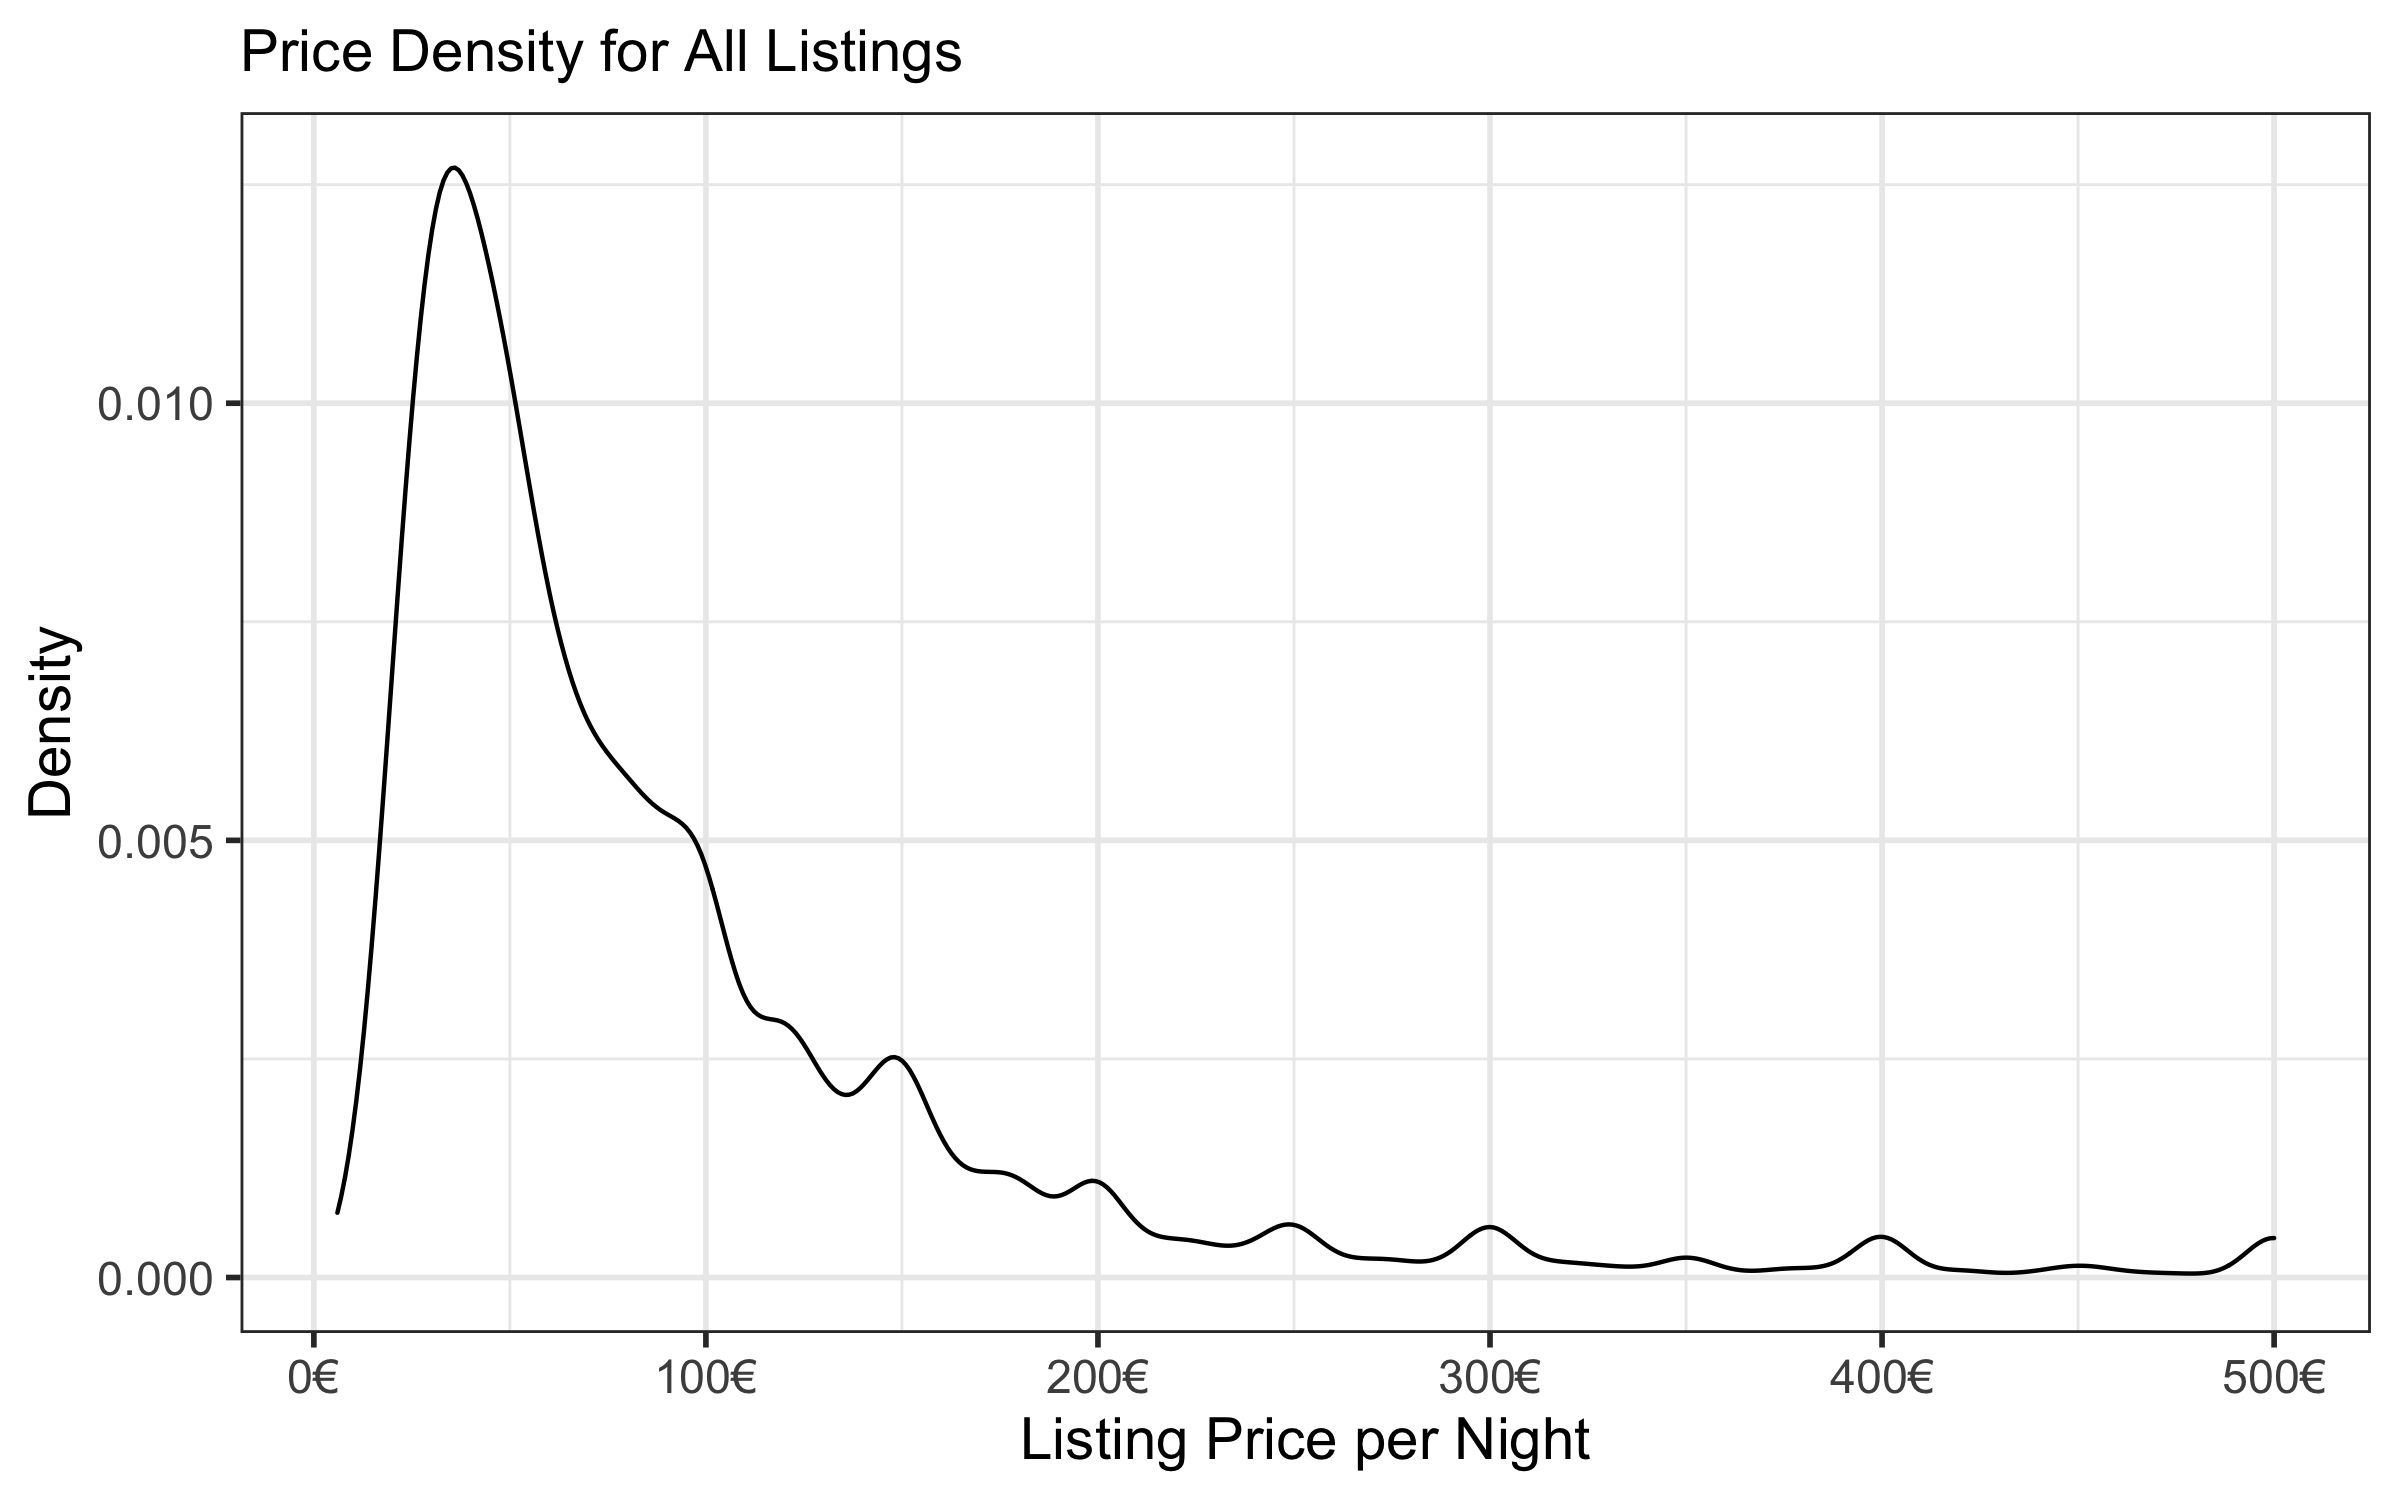
\includegraphics[width=6.77083in,height=\textheight]{../images/density_plot.png}
\caption{Density plot for prices of Airbnb listings in Barcelona, Spain:
Listings have an extreme positive skew and appear to be multimodal. The
modality reflects the tendency for listings to be priced in increments
of 50 Euros}
\end{figure}

\hypertarget{correlogram}{%
\paragraph{Correlogram}\label{correlogram}}

Based on the correlogram shown below there is little correlation between
the 6 numerical variables presented. All positive correlations are in
blue, and all negative correlations are in red.

\begin{figure}
\centering
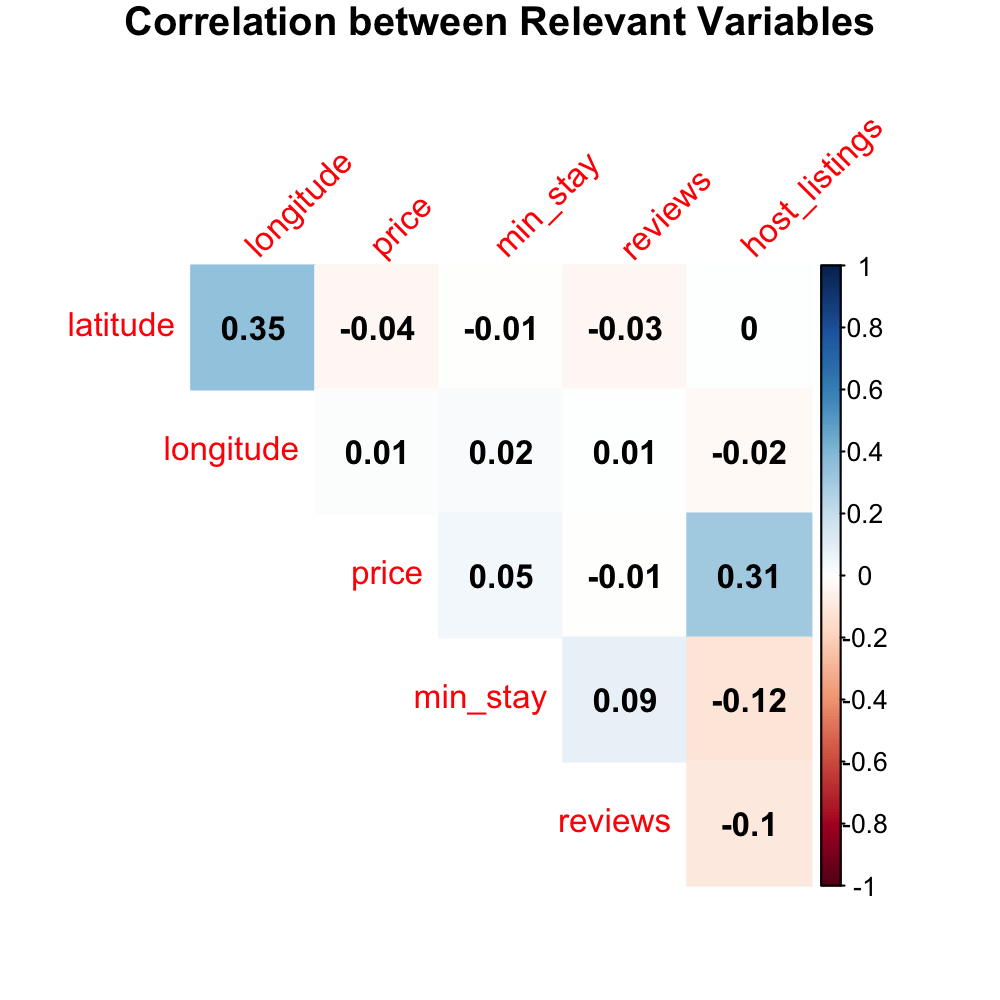
\includegraphics[width=5.20833in,height=\textheight]{../images/correlogram.png}
\caption{Correlations for potentially significant variables in the
explaining the price of Airbnb listings}
\end{figure}

\hypertarget{violin-plot}{%
\paragraph{Violin Plot}\label{violin-plot}}

The violin plot below shows the distribution of price in log10 scale for
each district in descending order of average price. Based on the plot,
Example has the highest priced and Nou Barris has the lowest priced
listings.

\begin{figure}
\centering
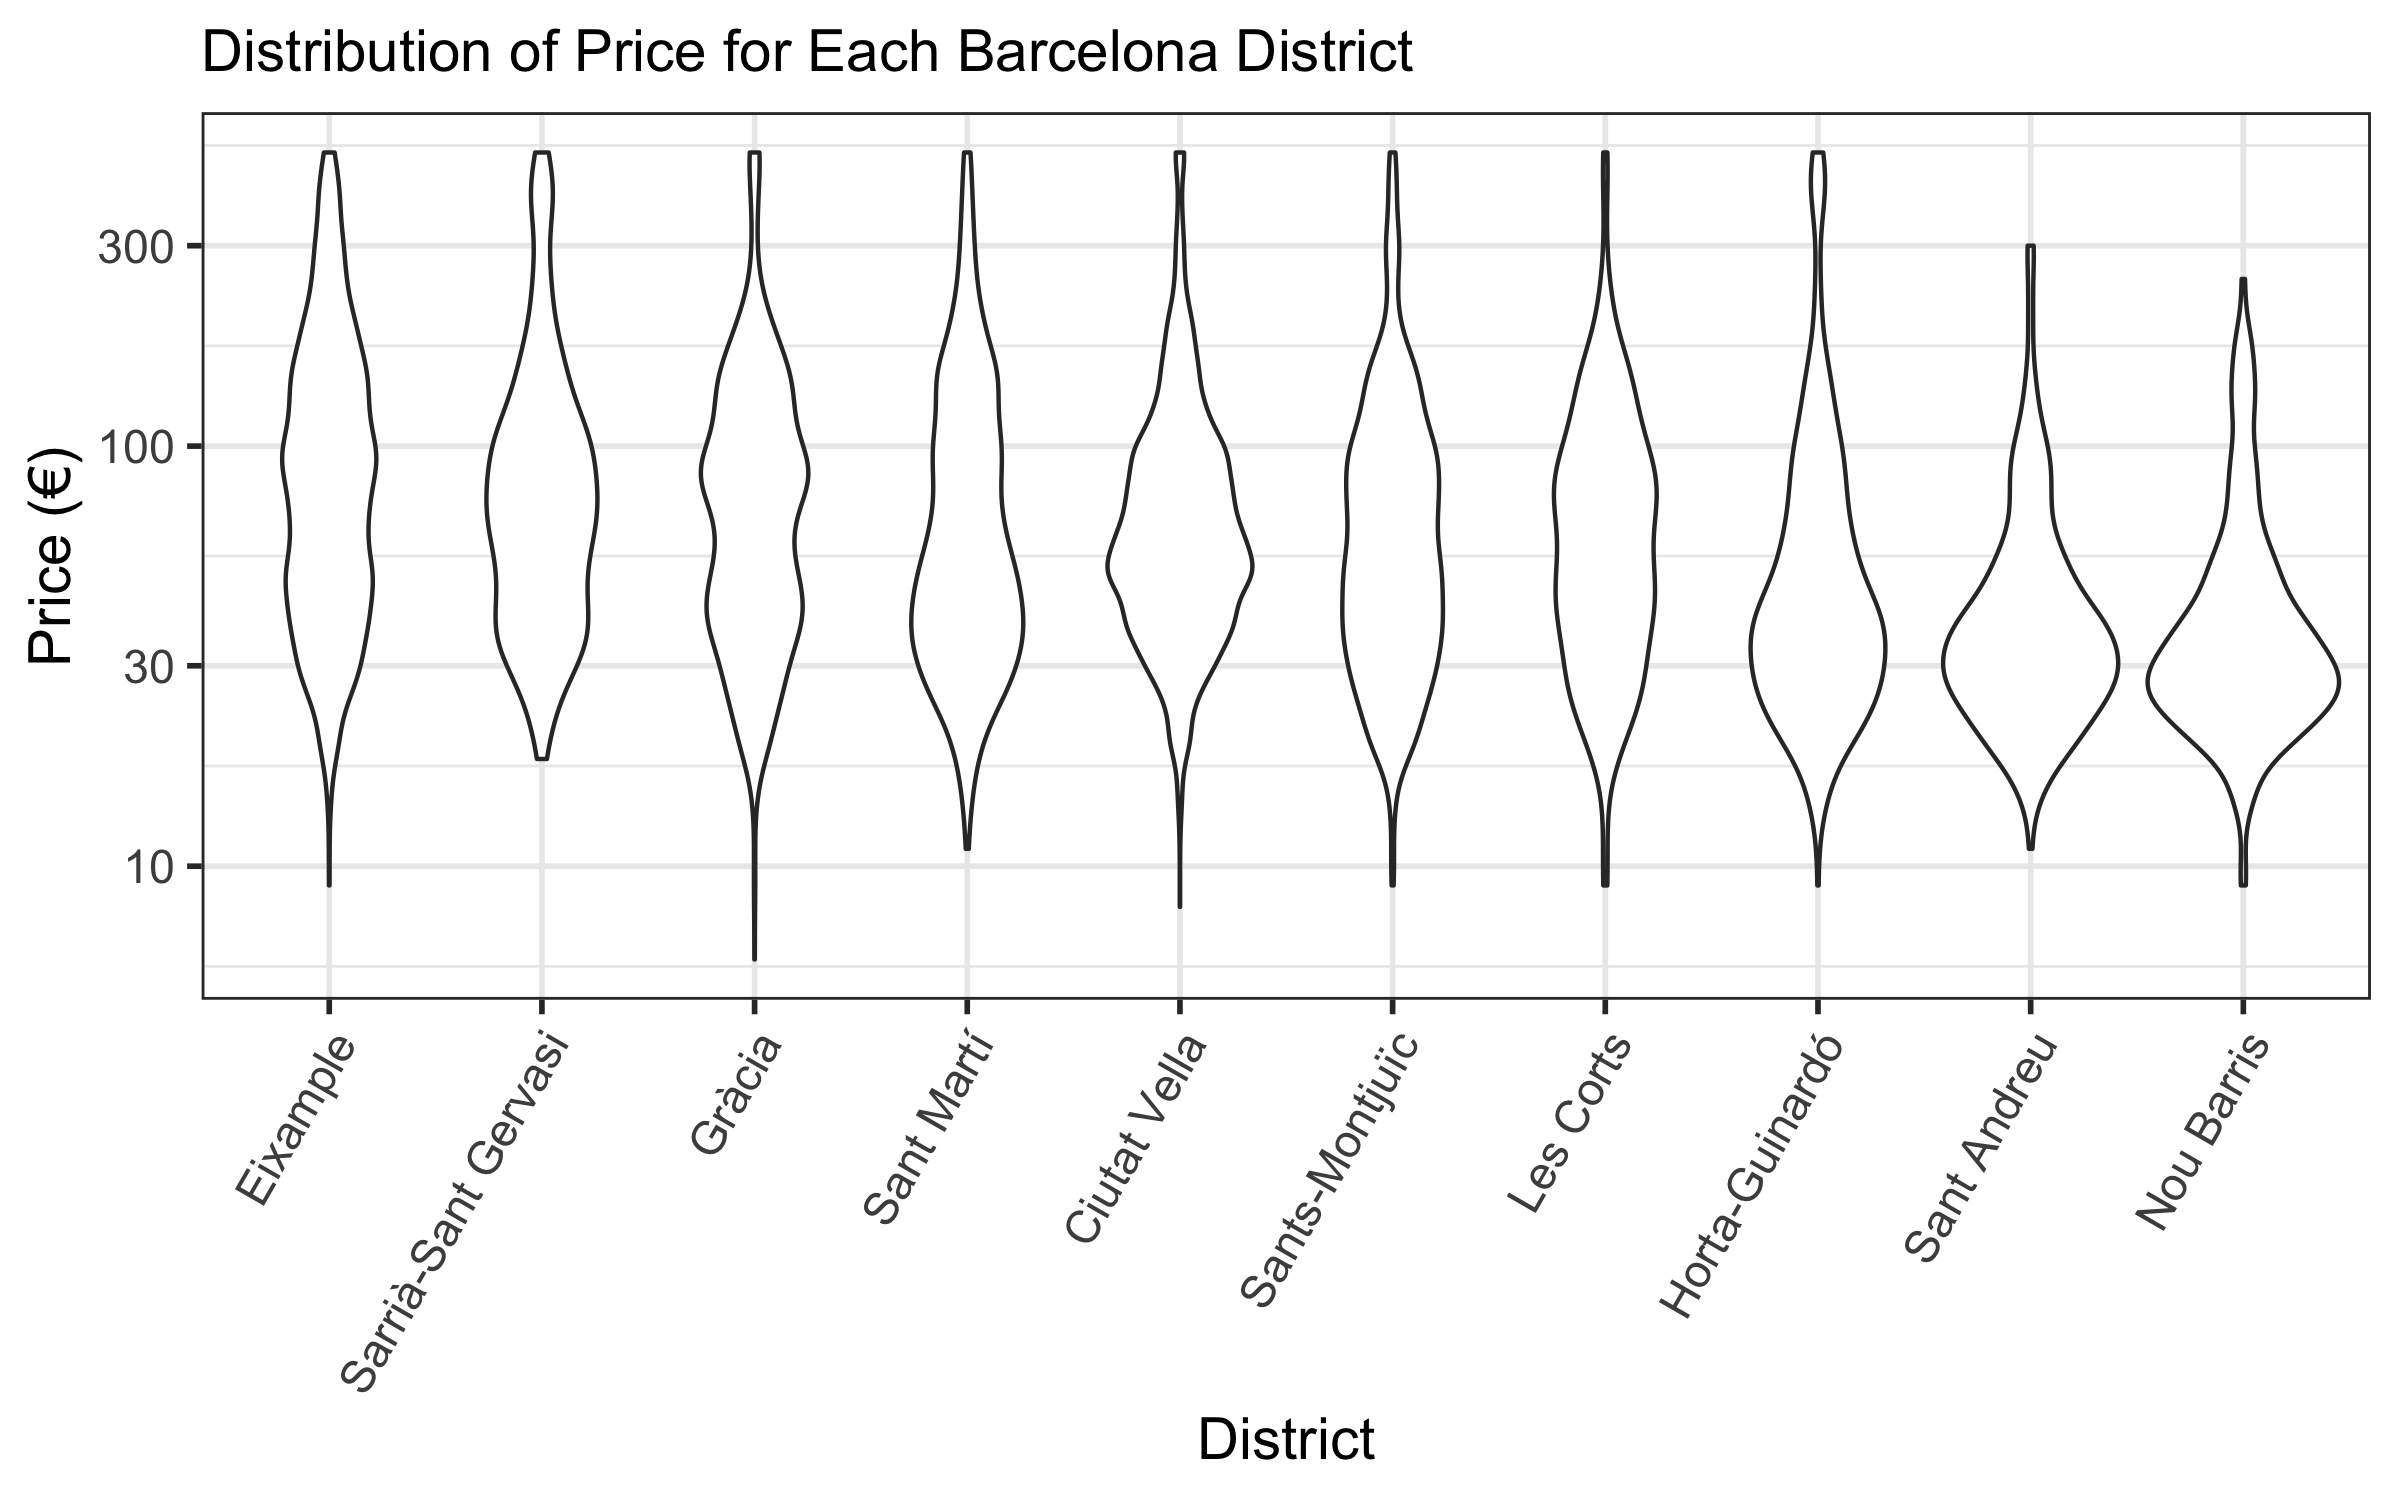
\includegraphics[width=7.03125in,height=\textheight]{../images/violin_plot.png}
\caption{Plot shows the distribution of listing prices for Airbnb
listings in Barcelona, Spain by city district}
\end{figure}

\hypertarget{analysis-methods}{%
\subsubsection{Analysis Methods}\label{analysis-methods}}

We perform linear regression on Airbnb listing prices to the listing's
district, type of room, reviews left per month, and distance from city
center to see how these variables might be affecting the Airbnb listing
prices in Barcelona. First, we run

\texttt{lm(price\ \textasciitilde{}\ district\ +\ room\_type\ +\ distance\ +\ reviews\_per\_month,\ data=df)}

where our data is housed in the dataframe, \texttt{df} and look at the
QQ-Plots of the standardized residuals. This plot is given as the left
plot below. It is obvious that normality assumptions are not
appropriate, so we then run

\texttt{lm(log(price)\ \textasciitilde{}\ district\ +\ room\_type\ +\ distance\ +\ reviews\_per\_month,\ data=df)}

and look at the QQ-plot for the log transform of price. This QQ-plot is
given below on the right and is much closer to the normality assumption
even though there is evidence of heavier tails.

\begin{figure}
\centering
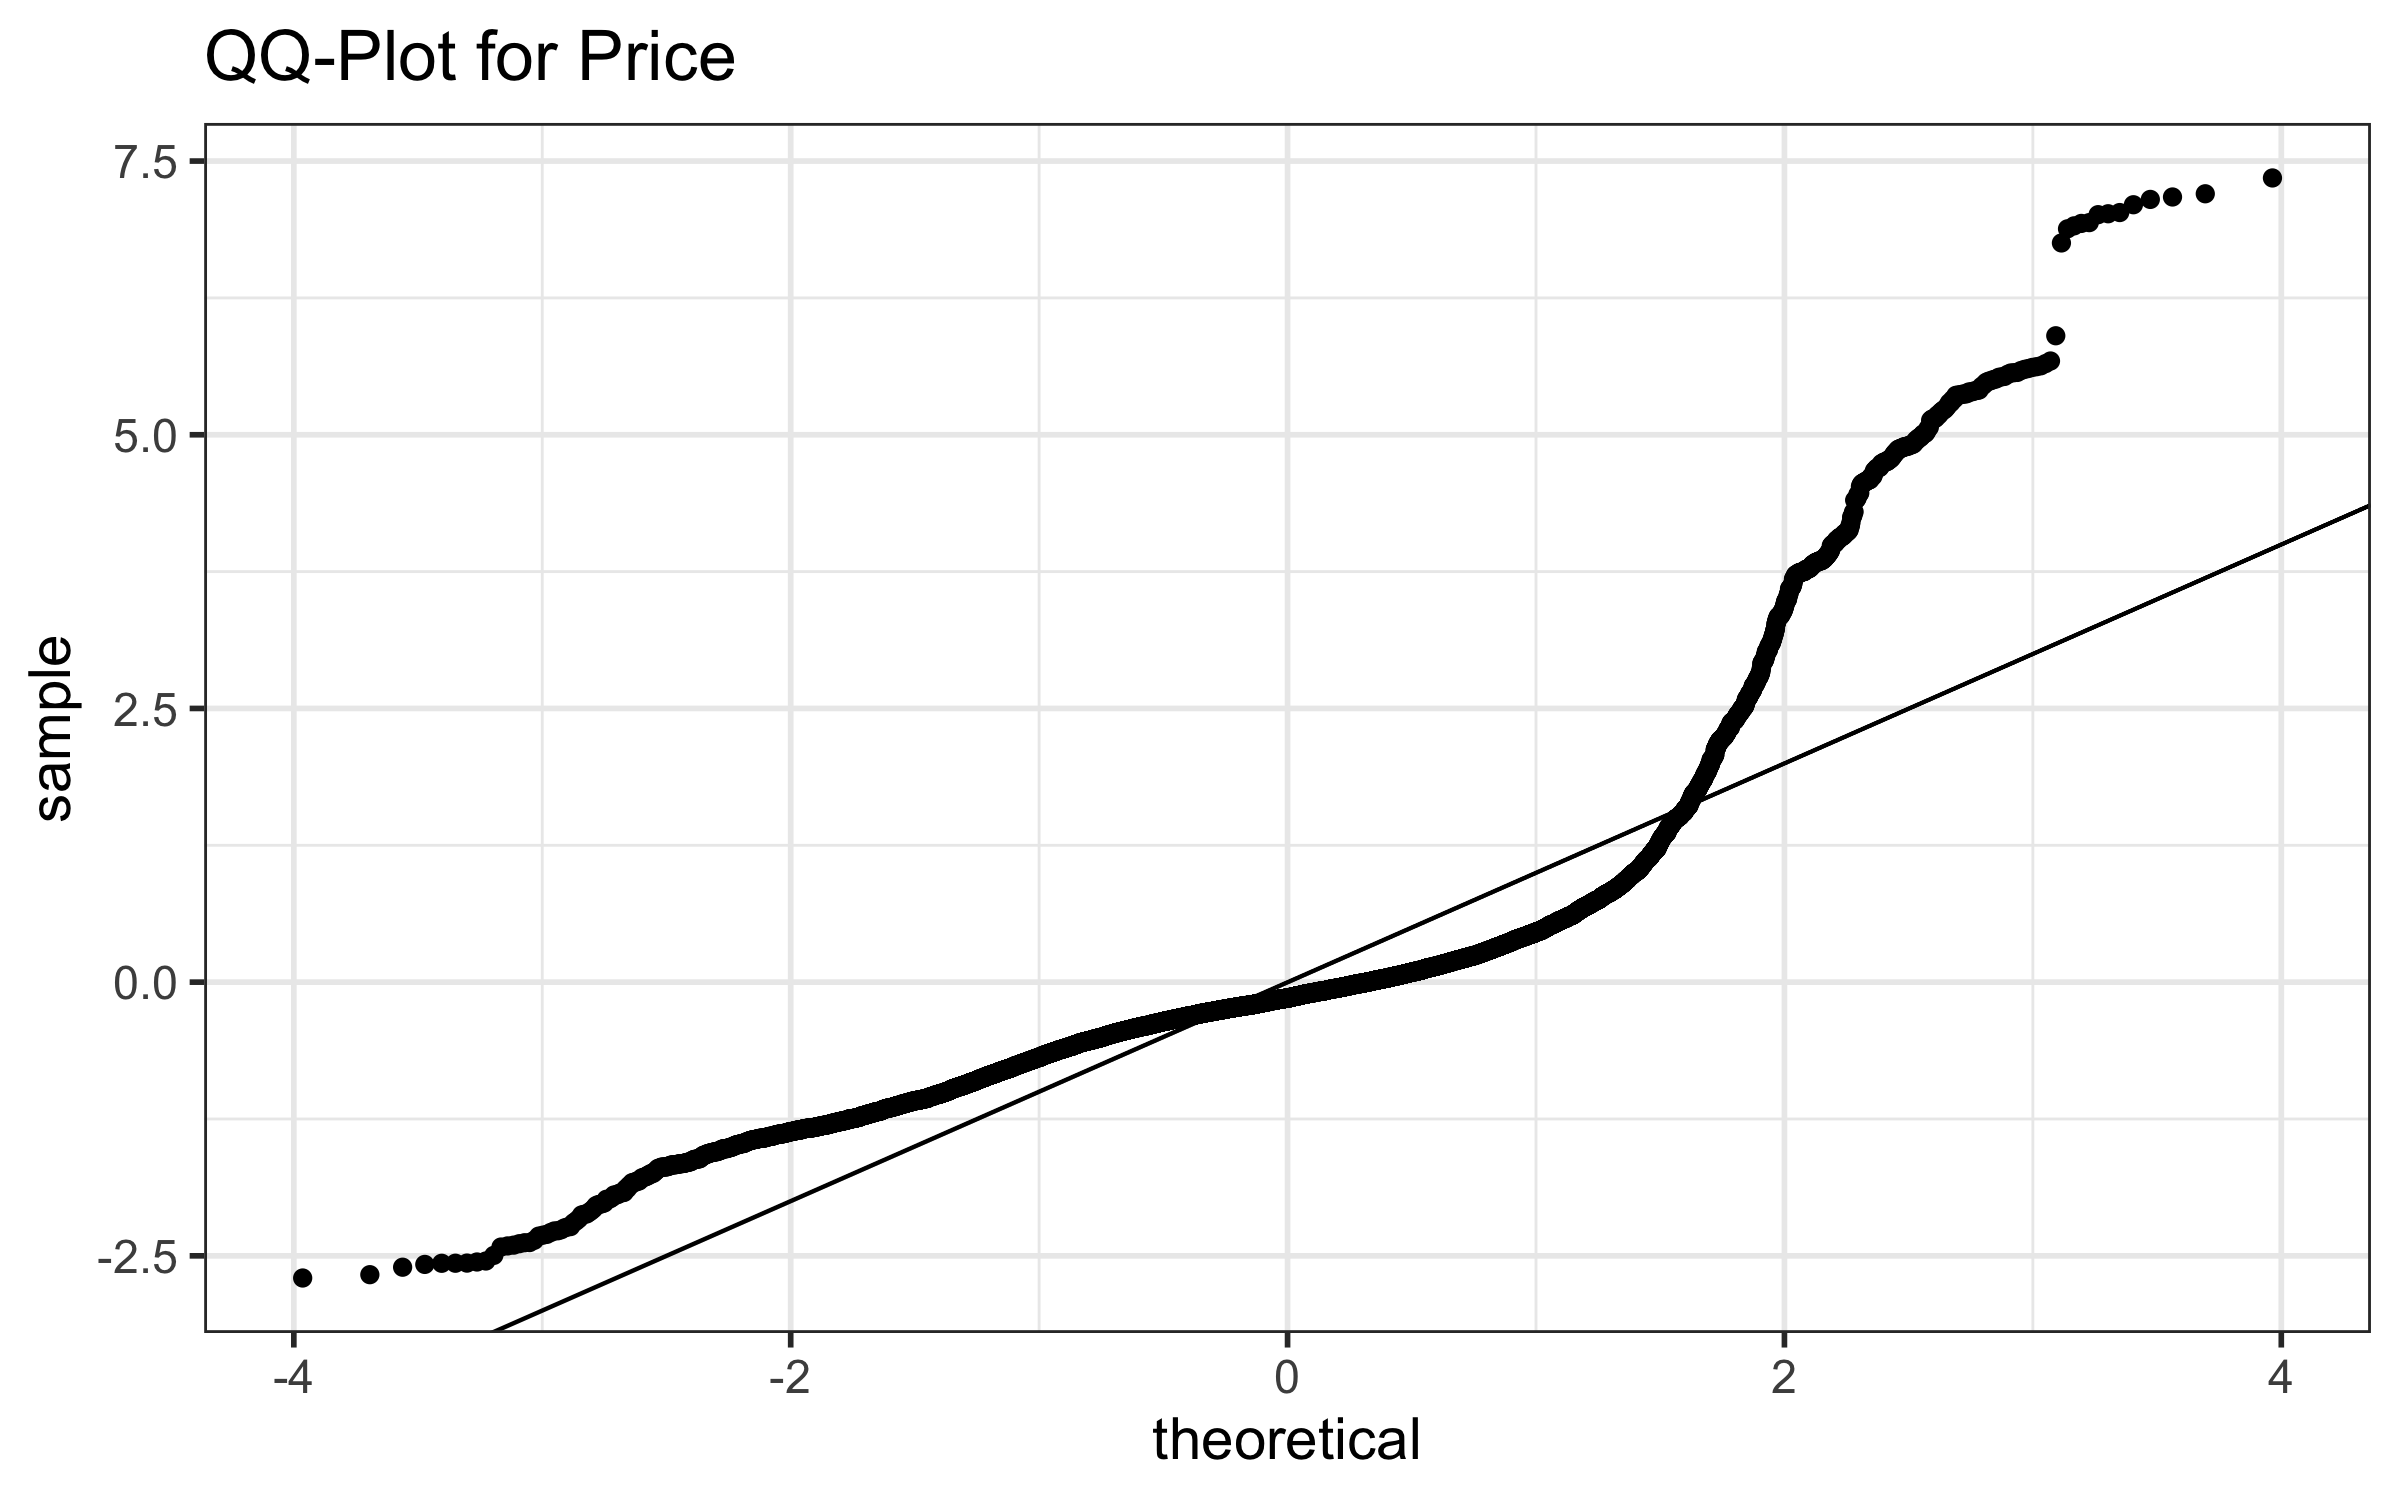
\includegraphics[width=6.25in,height=\textheight]{../images/lm1-QQPlot.png}
\caption{QQ-Plot for standardized residuals of the regression on the raw
price data: The residuals show evidence that the errors are not normally
distributed}
\end{figure}

\begin{figure}
\centering
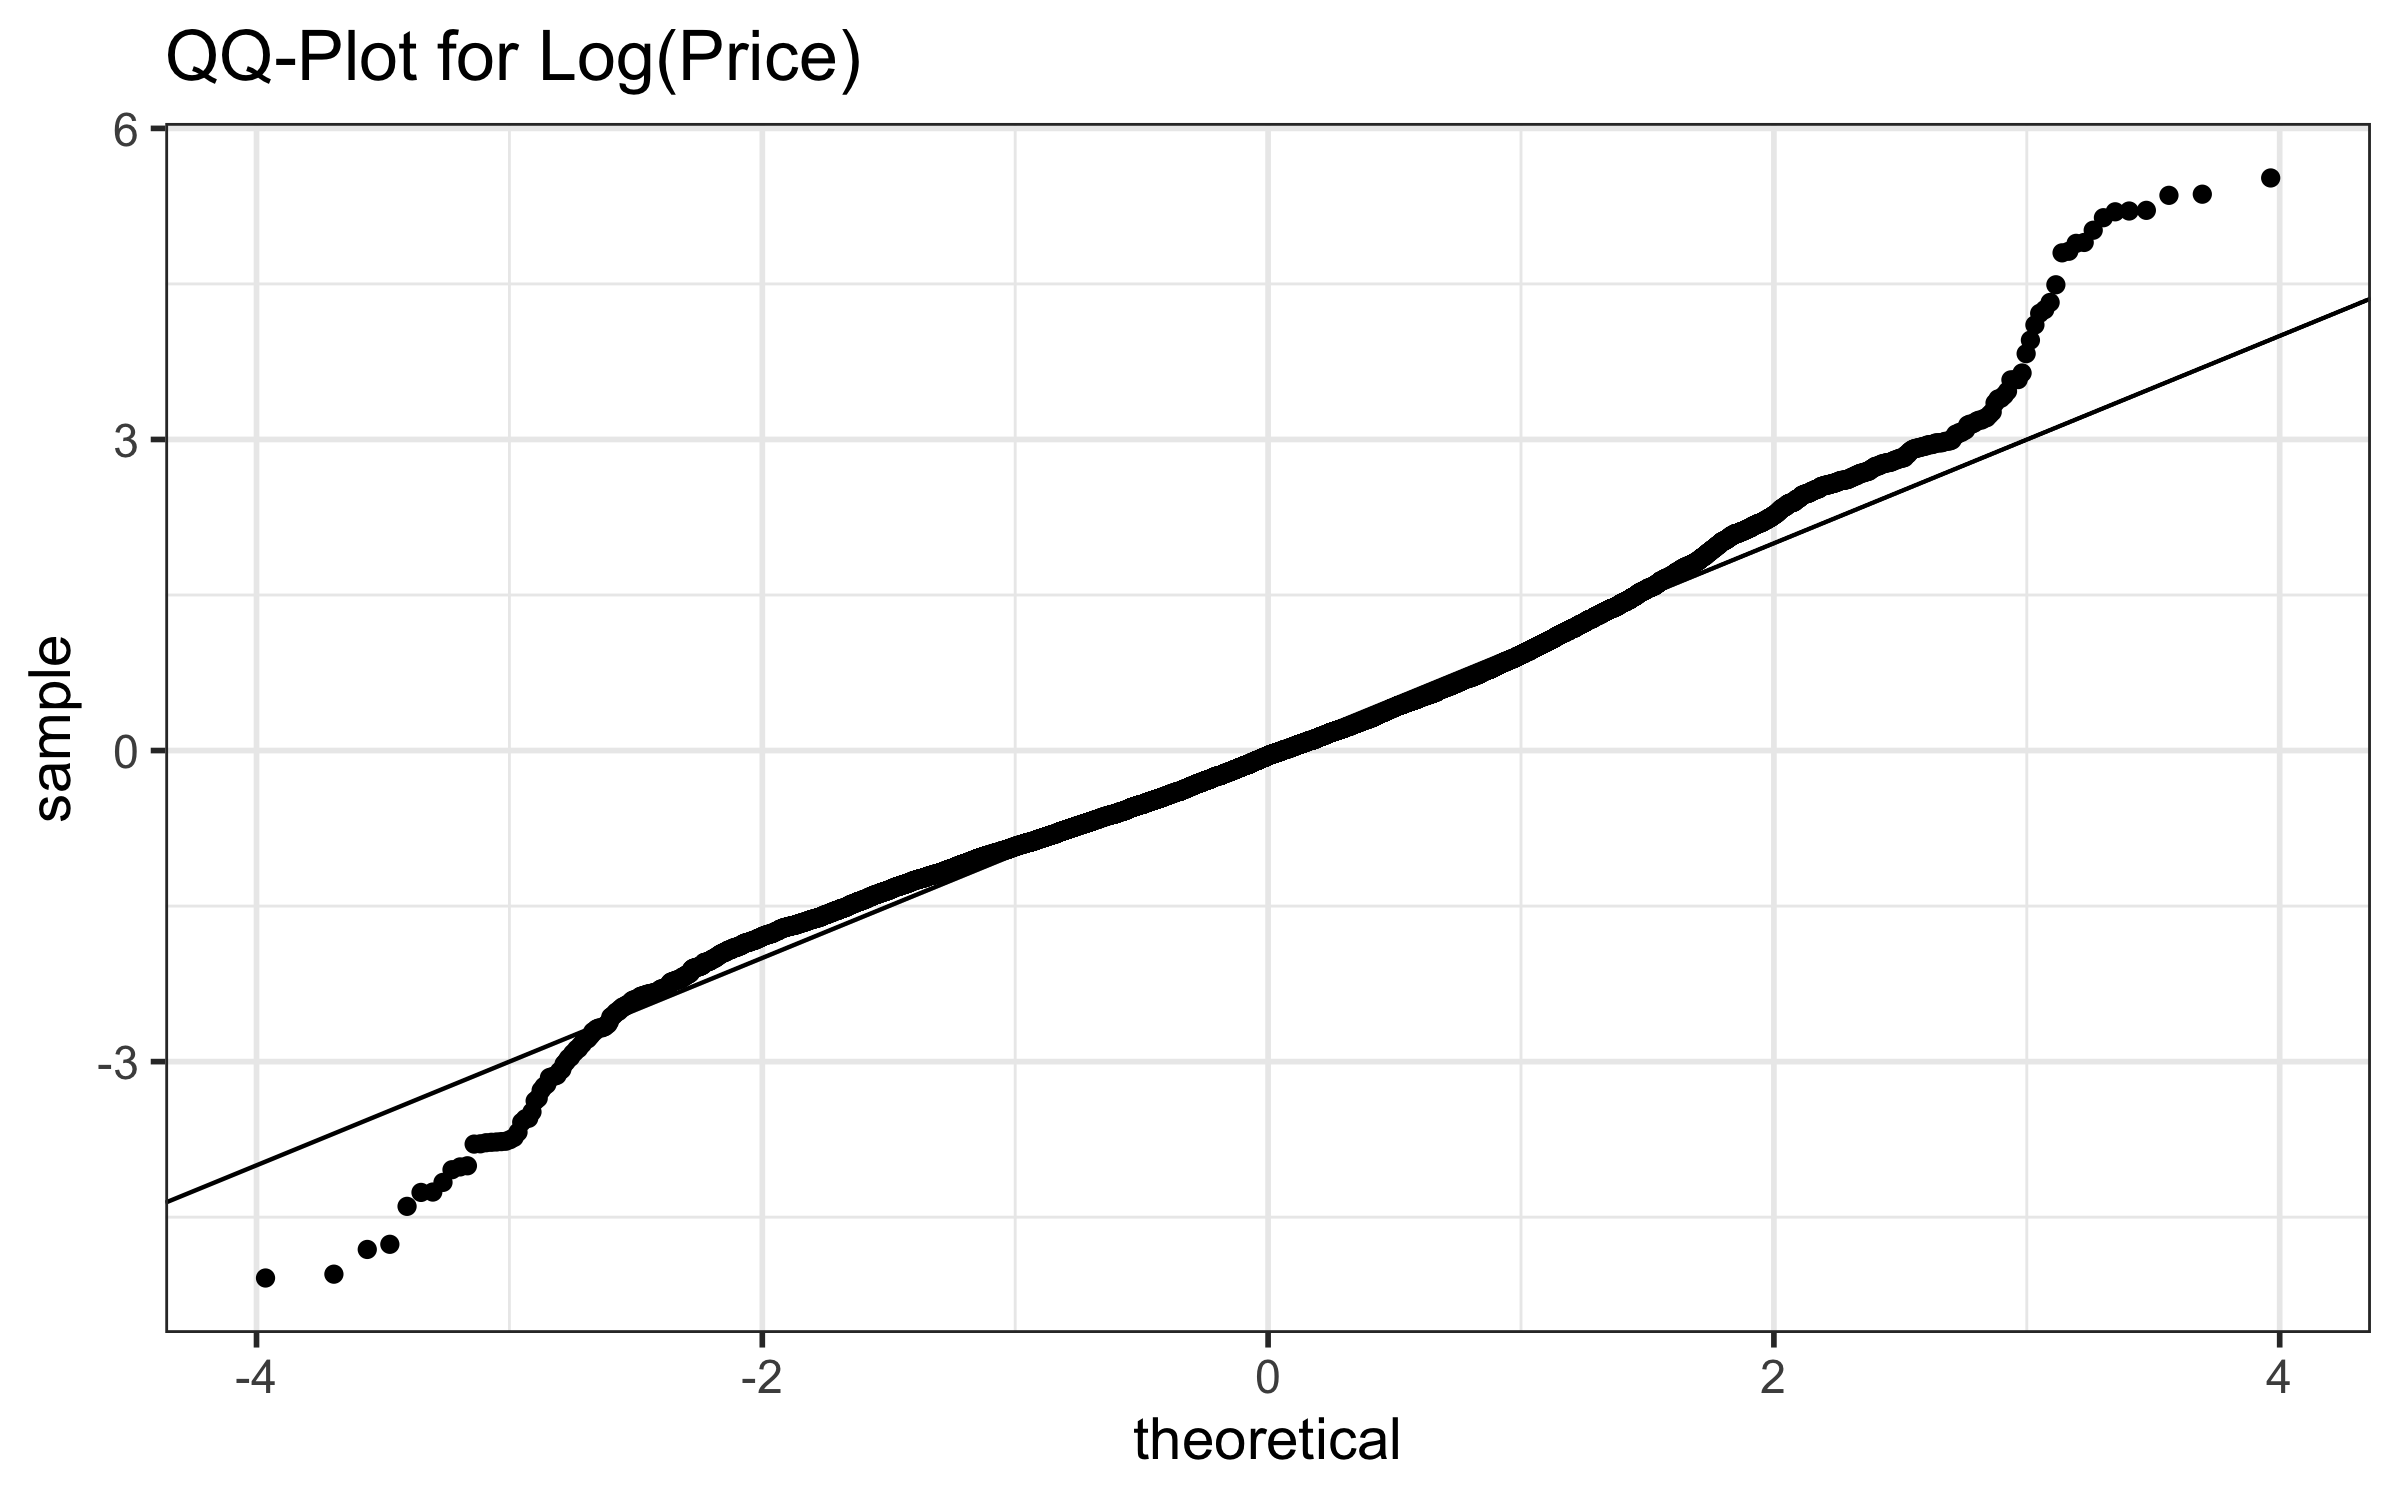
\includegraphics[width=6.25in,height=\textheight]{../images/lm2-QQPlot.png}
\caption{QQ-Plot for standardized residuals of the regression on the log
transform of price data: The residuals seem to have heavier tails than
the normal distribution, but are better suited for linear regression
than the untransformed price data}
\end{figure}

\hypertarget{analysis-results}{%
\subsubsection{Analysis Results}\label{analysis-results}}

First, let's look at the results of the linear regression for the
untransformed price response variable. In the output below, we see that
only 2 of the 10 districts, with Ciutat Vella as the base district, are
statistically significant at the 95\% confidence level. These are
Eixample and Sarrià-Sant Gervasi.

\begin{Shaded}
\begin{Highlighting}[]
\CommentTok{#Linear Model on Price}
\NormalTok{lm}\FloatTok{.1}\NormalTok{ <-}\StringTok{ }\KeywordTok{readRDS}\NormalTok{(}\DataTypeTok{file=}\NormalTok{here}\OperatorTok{::}\KeywordTok{here}\NormalTok{(}\StringTok{"data"}\NormalTok{, }\StringTok{"lm1_results.rds"}\NormalTok{))}
\KeywordTok{tidy}\NormalTok{(lm}\FloatTok{.1}\NormalTok{)}
\end{Highlighting}
\end{Shaded}

\begin{verbatim}
## # A tibble: 15 x 5
##    term                        estimate std.error statistic  p.value
##    <chr>                          <dbl>     <dbl>     <dbl>    <dbl>
##  1 (Intercept)                  154.        1.76     87.6   0.      
##  2 districtEixample              13.7       1.84      7.44  1.05e-13
##  3 districtGràcia                -0.959     2.80     -0.342 7.32e- 1
##  4 districtHorta-Guinardó         4.49      3.92      1.14  2.53e- 1
##  5 districtLes Corts              0.938     5.09      0.184 8.54e- 1
##  6 districtNou Barris             4.50      6.08      0.741 4.59e- 1
##  7 districtSant Andreu           -3.51      5.11     -0.687 4.92e- 1
##  8 districtSant Martí             4.21      2.49      1.69  9.02e- 2
##  9 districtSants-Montjuïc        -2.76      2.67     -1.03  3.02e- 1
## 10 districtSarrià-Sant Gervasi   18.2       4.20      4.33  1.48e- 5
## 11 room_typeHotel room           30.7       3.58      8.58  1.03e-17
## 12 room_typePrivate room        -89.9       1.20    -74.7   0.      
## 13 room_typeShared room         -92.5       6.85    -13.5   3.19e-41
## 14 distance                    -489.       68.2      -7.17  7.80e-13
## 15 reviews_per_month             -3.13      0.320    -9.80  1.40e-22
\end{verbatim}

We can interpret the estimate for Eixample, 13.7, as saying that prices
of Airbnb listings in the Eixample district differ from listings in the
Ciutat Vella district, on average, by 13.7 Euro's per night. All room
types, distance, and reviews per month are statistically significant at
any reasonable confidence level.

Next, we look at the results of the linear regression on the log(price)
of Airbnb listings. In the output below, we see many more districts are
now statistically significant, but the interpretation of their
coefficient estimates are not as straightforward as the results when
regressing on listing price.

\begin{Shaded}
\begin{Highlighting}[]
\CommentTok{#Linear Model on log(Price)}
\NormalTok{lm}\FloatTok{.2}\NormalTok{ <-}\StringTok{ }\KeywordTok{readRDS}\NormalTok{(}\DataTypeTok{file=}\NormalTok{here}\OperatorTok{::}\KeywordTok{here}\NormalTok{(}\StringTok{"data"}\NormalTok{, }\StringTok{"lm2_results.rds"}\NormalTok{))}
\KeywordTok{tidy}\NormalTok{(lm}\FloatTok{.2}\NormalTok{)}
\end{Highlighting}
\end{Shaded}

\begin{verbatim}
## # A tibble: 15 x 5
##    term                        estimate std.error statistic   p.value
##    <chr>                          <dbl>     <dbl>     <dbl>     <dbl>
##  1 (Intercept)                   4.98     0.0137    363.    0.       
##  2 districtEixample              0.0771   0.0144      5.36  8.49e-  8
##  3 districtGràcia               -0.0280   0.0219     -1.28  2.00e-  1
##  4 districtHorta-Guinardó       -0.107    0.0306     -3.48  4.99e-  4
##  5 districtLes Corts             0.0537   0.0398      1.35  1.77e-  1
##  6 districtNou Barris           -0.0810   0.0475     -1.71  8.79e-  2
##  7 districtSant Andreu          -0.181    0.0399     -4.53  5.90e-  6
##  8 districtSant Martí           -0.0238   0.0194     -1.22  2.21e-  1
##  9 districtSants-Montjuïc       -0.0706   0.0209     -3.38  7.26e-  4
## 10 districtSarrià-Sant Gervasi   0.177    0.0328      5.39  7.11e-  8
## 11 room_typeHotel room          -0.0167   0.0280     -0.598 5.50e-  1
## 12 room_typePrivate room        -1.01     0.00940  -108.    0.       
## 13 room_typeShared room         -1.27     0.0536    -23.7   9.59e-122
## 14 distance                     -6.25     0.533     -11.7   1.28e- 31
## 15 reviews_per_month            -0.0214   0.00250    -8.57  1.18e- 17
\end{verbatim}

Due to the improved QQ-Plot for the log(price) model, we only consider
this model's results going forward. We can look at how well this model
fits the data by randomly selecting 10 listings and comparing the price
to the fitted price.

\begin{Shaded}
\begin{Highlighting}[]
\KeywordTok{set.seed}\NormalTok{(}\DecValTok{100}\NormalTok{)}
\KeywordTok{augment}\NormalTok{(lm}\FloatTok{.2}\NormalTok{) }\OperatorTok\StringTok{ }
\StringTok{  }\KeywordTok{slice}\NormalTok{(}\KeywordTok{sample}\NormalTok{(}\DecValTok{1}\OperatorTok{:}\KeywordTok{nrow}\NormalTok{(}\KeywordTok{augment}\NormalTok{(lm}\FloatTok{.2}\NormalTok{)), }\DataTypeTok{size=}\DecValTok{10}\NormalTok{, }\DataTypeTok{replace=}\OtherTok{FALSE}\NormalTok{)) }\OperatorTok\StringTok{ }
\StringTok{  }\KeywordTok{select}\NormalTok{(.rownames, district, room_type, distance, reviews_per_month, log.price., .fitted) }\OperatorTok\StringTok{ }
\StringTok{  }\KeywordTok{rename}\NormalTok{(}\DataTypeTok{price =}\NormalTok{ log.price.,}
         \DataTypeTok{fitted =}\NormalTok{ .fitted) }\OperatorTok\StringTok{ }
\StringTok{  }\KeywordTok{mutate}\NormalTok{(}\DataTypeTok{price =} \KeywordTok{exp}\NormalTok{(price),}
         \DataTypeTok{fitted =} \KeywordTok{exp}\NormalTok{(fitted))}
\end{Highlighting}
\end{Shaded}

\begin{verbatim}
## # A tibble: 10 x 7
##    .rownames district        room_type    distance reviews_per_mon~ price fitted
##    <chr>     <chr>           <chr>           <dbl>            <dbl> <dbl>  <dbl>
##  1 4036      Ciutat Vella    Entire home~   0.0123             0.02 135.   134. 
##  2 514       Eixample        Entire home~   0.0135             0.56 149    142. 
##  3 3623      Sarrià-Sant Ge~ Private room   0.0404             3.27  84.0   45.5
##  4 3935      Ciutat Vella    Private room   0.0110             0.13  40     49.0
##  5 4375      Sant Andreu     Entire home~   0.0331             1.16  60.0   95.9
##  6 8530      Eixample        Private room   0.0297             0.27  50.0   46.9
##  7 3190      Eixample        Entire home~   0.0226             0.12  85.   136. 
##  8 12181     Sant Martí      Entire home~   0.0284             4.02 180    109. 
##  9 8849      Eixample        Private room   0.0173             3.33  55.    47.5
## 10 9365      Sants-Montjuïc  Entire home~   0.0218             0.47 120.   117.
\end{verbatim}

In the output above, the \texttt{price} columns shows the listing's
price from the Airbnb website and \texttt{fitted} shows the price given
by the linear model. Note that we exponentiated this output so that it
is in Euro's and straightforward to compare.

Finally, we can look at the adjusted r-squared to see how much of the
variance in listing price is explained by district, type of room,
distance of city center, and reviews per month. By using the
\texttt{glance()} function from the \texttt{broom} package, we see that
52.36\% of the variance of the log transform of listing is explained by
our model.

\hypertarget{discussion}{%
\subsubsection{Discussion}\label{discussion}}

Based on the results of our model using the log transform of listing
price, district, type of room, distance from city center, and reviews
per month all play a significant role in the price of an Airbnb listing.
However, much of the variance is left unexplained in our model so that
we may want to look for additional variables.

\hypertarget{references}{%
\subsubsection{References}\label{references}}

\href{http://insideairbnb.com/get-the-data.html}{Airbnb dataset}

\end{document}
